\section{Żadanie adresacji}
Tutaj po raz pierwszy można zaobserwować zmienioną wartość pola adresu dla wiadomości
przychodzącej. Oznacza to, że urządzenie podrzędne zaakceptowało żadanie adresacji 
oraz identyfikuje się w trakcie rozmowy z urządzeniem nadrzędnym pod adresem 0x03 co
jest prawdą dla każdej następnej wiadomości.
\newline\newline
Budowa ramki wysyłanej przez tę komendę jest bardzo podobna do powyższej z racji tego, że powyższą można nazwać atrapą skanu a tą skanowaniem celowanym.
Z racji tego, że różna jest liczba oraz wielkość poszczególnych parametrów HDLC, bajt rozmiaru grupy posiada wartość 0x11.
\newline
Pierwszy parametr identyfikuje się przy pomocy wartości 0x01 czyli jest to unikalny identyfikator urządzenia, który ma zostać zaadresowany.
Kolejny bajt przypomina o rozmiarze parametru i w tym przypadku jest on równy 0x09. W powyższym opisie przedstawiono unikalny identyfikator urządzenia, który w przypadku
równości z rzeczywistym, pozwala urządzeniu podrzędnemu przyjąć żądanie adresacji.
\newline
Następny parametr posiada wartość 0x02 i oznacza on, że w jego wartości urządzenie nadrzędne zdefiniowało adres urządzeniu wewnetrznemu, dzięki któremu
będzie identyfikowane oraz z racji tego, że długość parametru ma wartość 0x01, to wartość wynosi 0x03. W przypadku obecnej pracy, nie będzie miał on większego znaczenia
aczkolwiek w momencie kiedy urządzenia typu Ret połączone są ze sobą szerogowo, potrzeba jest możliwość wysłania wiadomości do na przykład drugiego w łańcuchu.
\newline
Wartość ostatniego parametru równa 0x04, definiuje typ urządzenia podrzędnego, z którym inicjalizowana jest komunikacja. Długość wynosi 0x01 a wartość to 0x01.
Oznacza ona, że podejmowana jest próba nawiązania komunikacji z pojedyncznym RET-em.
Dla porównania istnieją również urządzenia takie jak MultiRET, dzięki któremu można zmieniać wartość nachylania kąta głównej wiązki anteny na wielu osiach czy płaszczyznach.


identyfikujące się unikalnym identyfikatorem \textit{UniqueID} == \{0x4E, 0x4B, 0x34, 0x36, 0x35, 0x30, 0x30, 0x30, 0x30\}
\begin{figure}[h!]
    \centering
    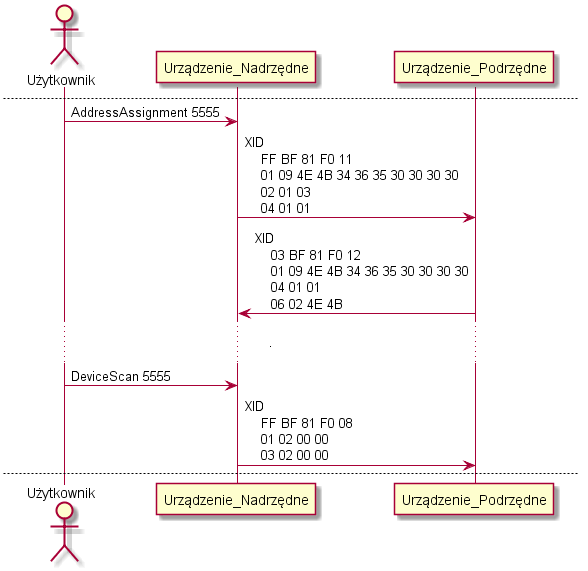
\includegraphics[scale=0.75]{out/Diagramy/UML_DiagramOfSequence_New/UML_DiagramOfSequence_New-page2.png}
    \caption{Żadanie adresacji oraz dodatkowe skanowanie urządzeń.
        \newline(Opracowanie własne)}
    \label{fig:DiagramSequence_AddressAssignment_SecondDeviceScan}
\end{figure}
